%\chapter{Testing and Experimental Results}\label{ch:testing-and-experimental-results}
%\justify
%
%Product development has been completed for the project, and as a result, all functionalities have been thoroughly tested.
%This chapter presents a comprehensive overview of the features tested, providing screenshots and photographs of hardware to illustrate the outcome of the build systems.
%
%\section{Testing Methodology}\label{sec:testing-methodology}
%
%The testing phase involved various methodologies to ensure the functionality, performance, and reliability of Open-source Intelligence Data Mining System and  \("\)Call One\("\) caller ID  android app.
%The following testing methods were employed:
%
%\begin{enumerate}[label=\roman*.]
%    \item \textbf{Unit Testing:} Testing individual modules and components to verify their correctness and functionality.
%    Jest a Node.js module is used to test the components of the android app and call one app's backend.
%
%    \item \textbf{Testing and Debugging}: Used flipper to test the state of the application in different phase and checking shared preferences.
%
%    \item \textbf{Performance Testing:} Assessing the app's performance under various load conditions.
%    Used FlatList to render contacts and call logs to improve the performance.
%    As showing in the Figure~\ref{fig: Performance Testing} the performance score is 91 and on average it is rendering 57 frames per second.
%
%\end{enumerate}
%
%\begin{figure}[h]
%    \centering
%    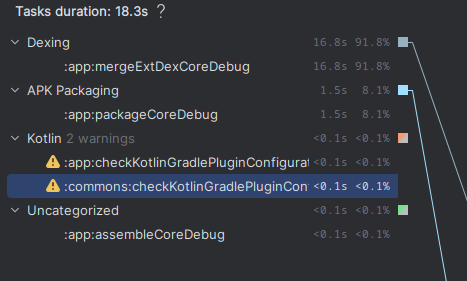
\includegraphics[width=1\linewidth]{Media/img}
%    \caption{App}
%    \label{fig:app-building}
%\end{figure}
%
%
%\begin{figure}
%    \centering
%    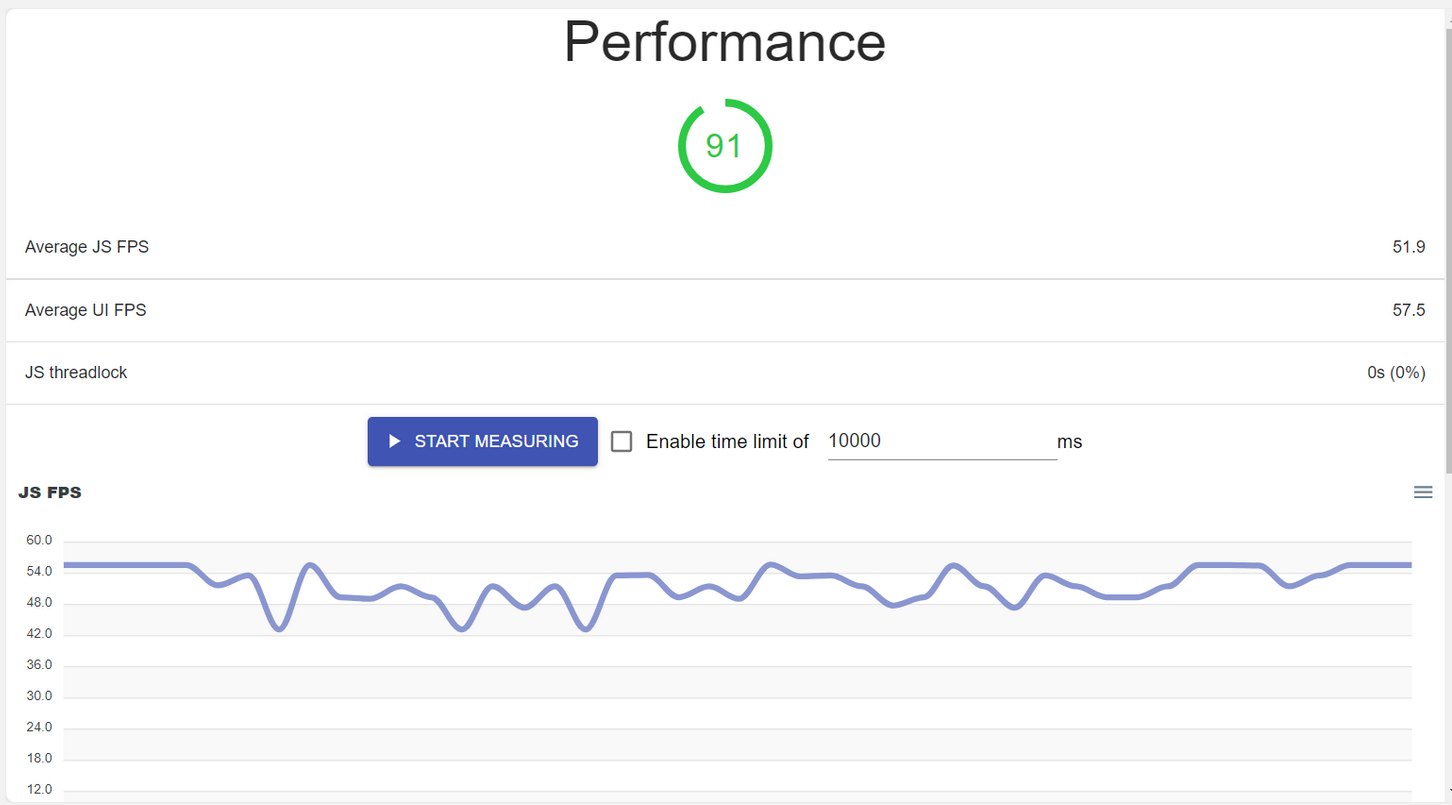
\includegraphics[width=1\linewidth]{Media//Chapter 6/performance}
%    \caption{Performance Testing}
%    \label{fig: Performance Testing}
%\end{figure}
%
%\section{App Building}\label{sec:app-building}
%
%The process of preparing an application for device deployment includes development, compiling, dexing, APK packing, and Kotlin:
%
%\begin{itemize}
%    \item \textbf{Development:} Coding and designing user interface features.
%    \item \textbf{Compiling:} Source code conversion into executable bytecode.
%    \item \textbf{Dexing:} Android-specific .class to .dex file conversion.
%    \item \textbf{APK Packing:} Final app assembly into a downloadable file.
%\end{itemize}
%
%\section{Experimental Results}\label{sec:experimental-results}
%
%The experimental results of the testing phase demonstrated the following outcomes:
%
%\begin{enumerate}[label=\roman*.]
%    \item \textbf{Functionalities Verified:} All functionalities of the \("\)Call One\("\) app were verified and found to be working as expected.
%
%    \item \textbf{Performance Optimization:} Performance testing revealed that the app performs optimally under various load conditions, ensuring smooth user experience.
%
%\end{enumerate}
%
%After conducting the tests, all the test cases had been passed, the bugs had been fixed, and it's ready to be released.
%The flow of testing and fixing the bugs is depicted in the figure.
%
%\section{Screenshots and Photographs}\label{sec:screenshots-and-photographs}
%
%Visual representations of the tested features, user interface, and hardware setup are provided below for reference and illustration.
%
%\begin{figure}
%    \centering
%    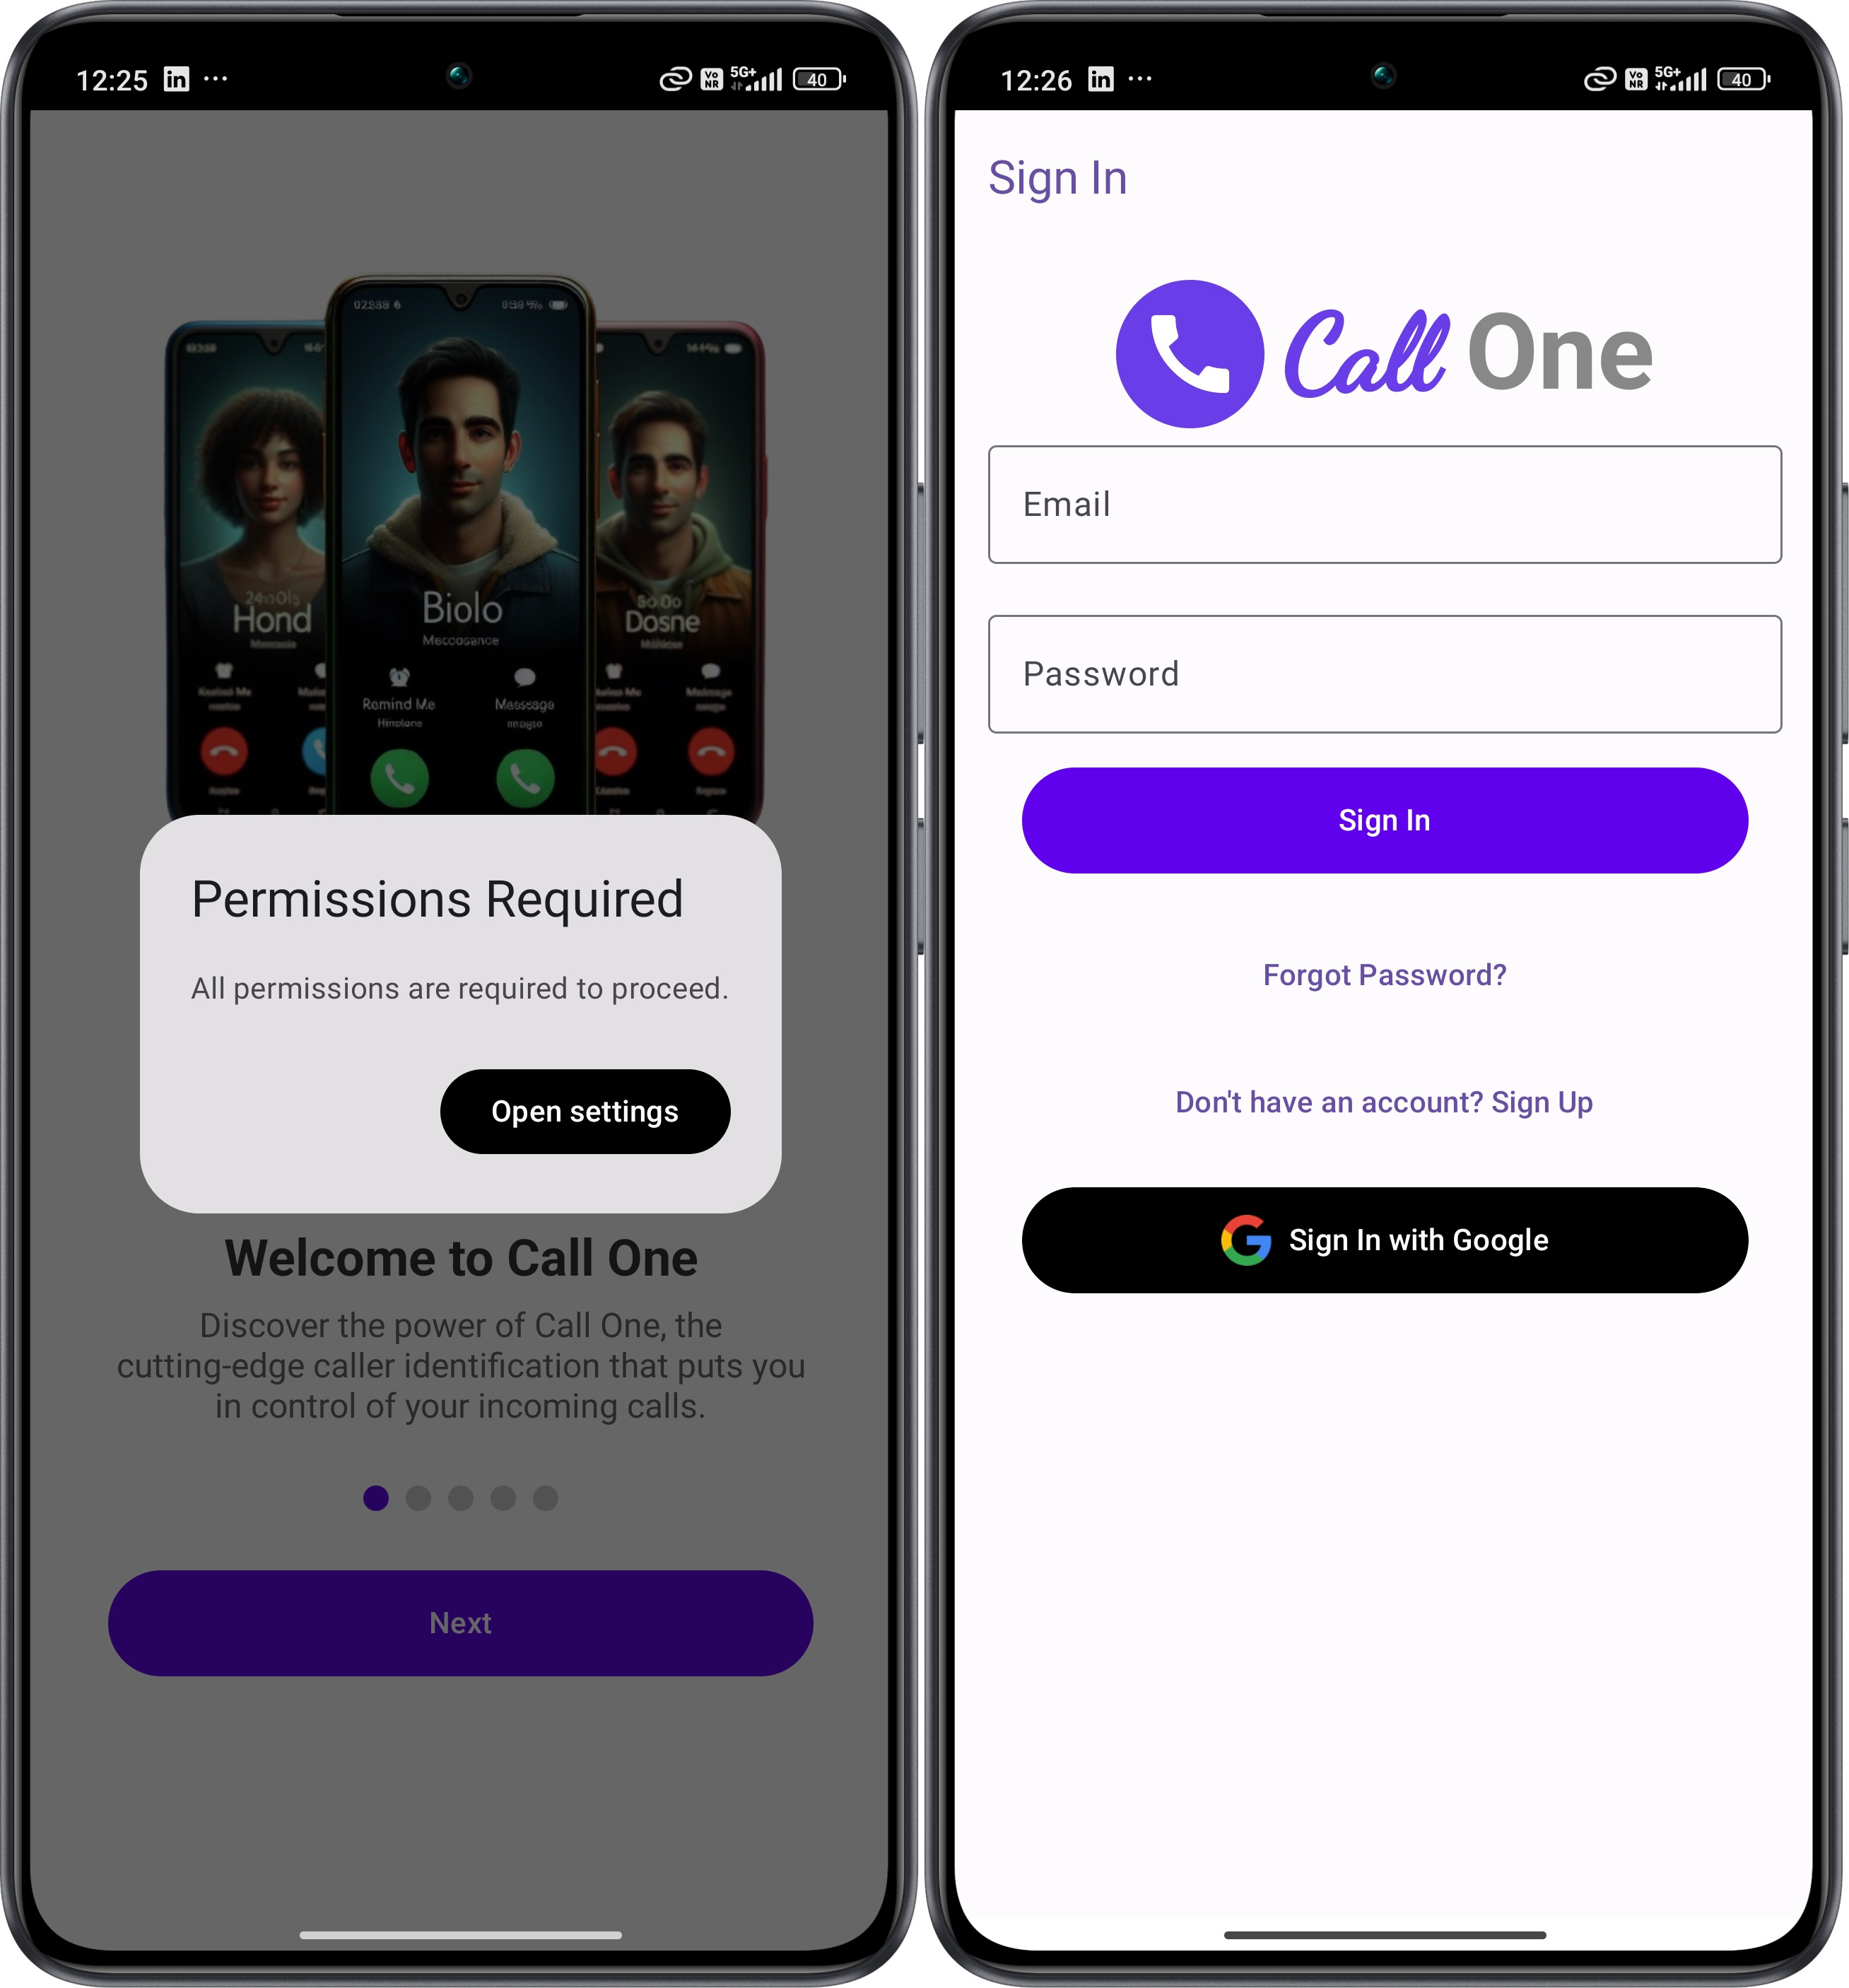
\includegraphics[width=1\linewidth]{Media//whatsapp/signin}
%    \caption{Call One App SignIn Screen}
%    \label{fig:Call One App SignIn Screen}
%\end{figure}
%
%\begin{figure}
%    \centering
%    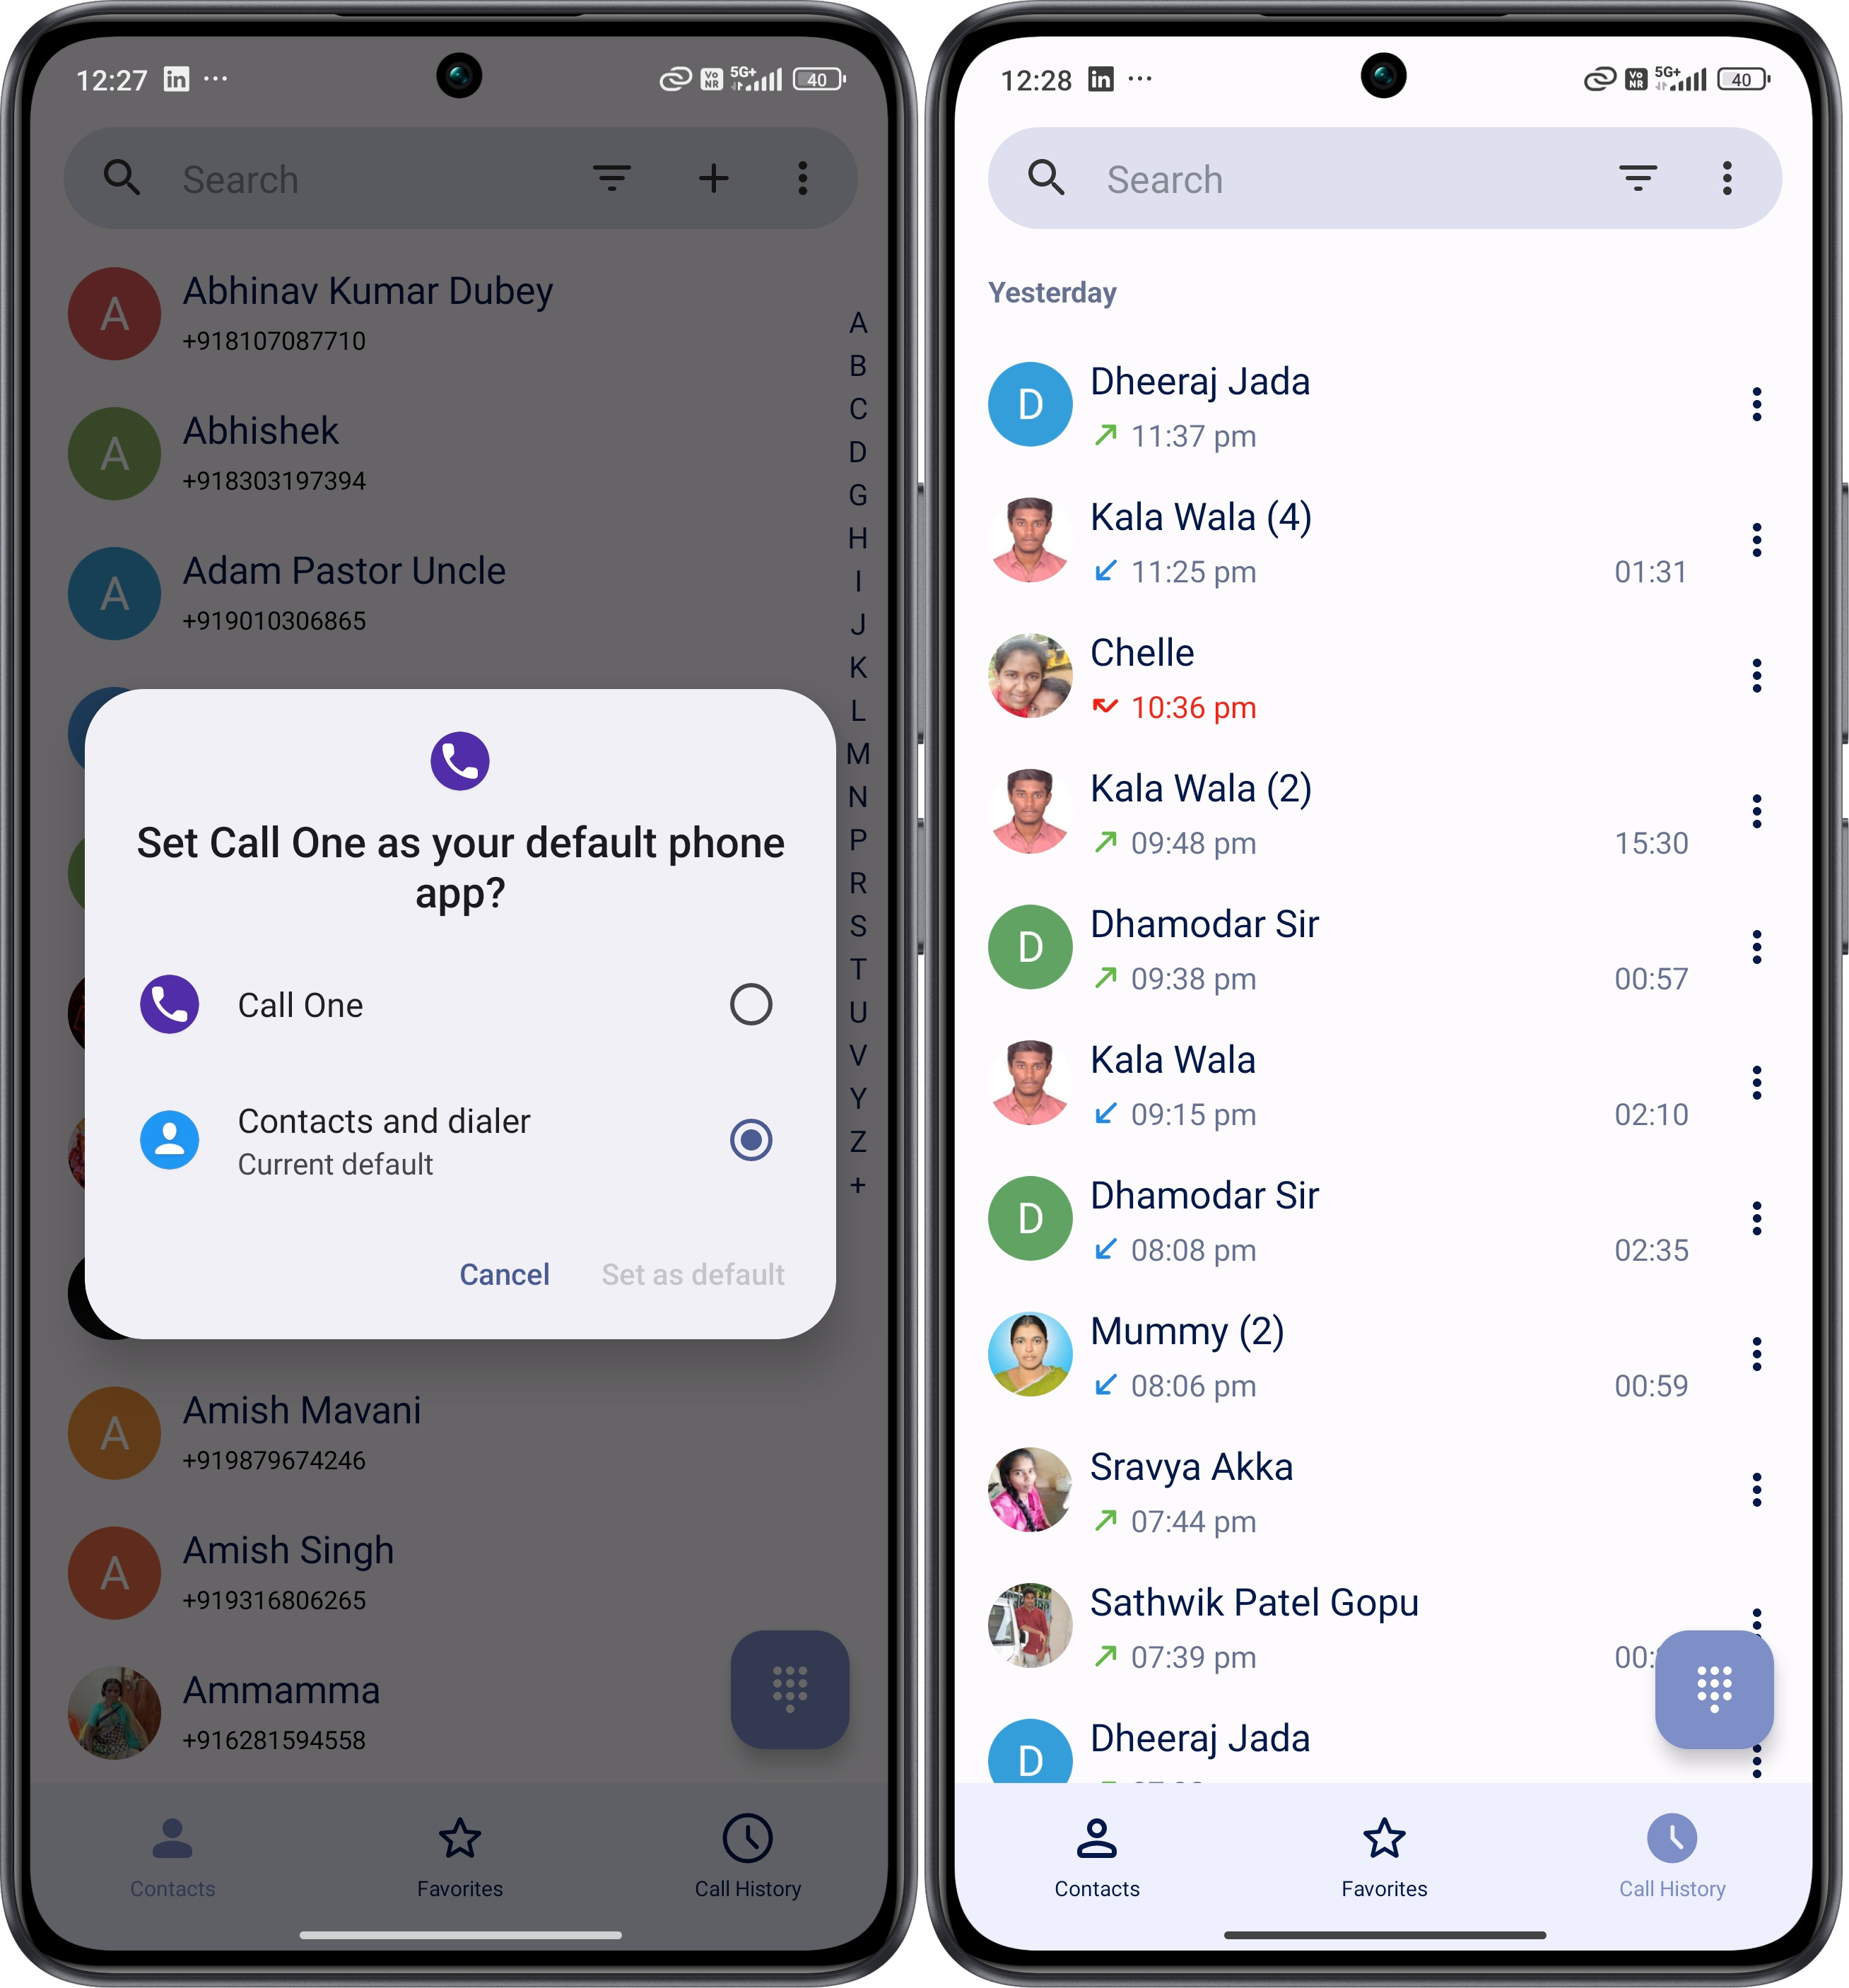
\includegraphics[width=1\linewidth]{Media//whatsapp/dd}
%    \caption{Default Dialer Setup and Call Logs Tab}
%    \label{fig:Default Dialer Setup and Call Logs Tab}
%\end{figure}
%
%\begin{figure}
%    \centering
%    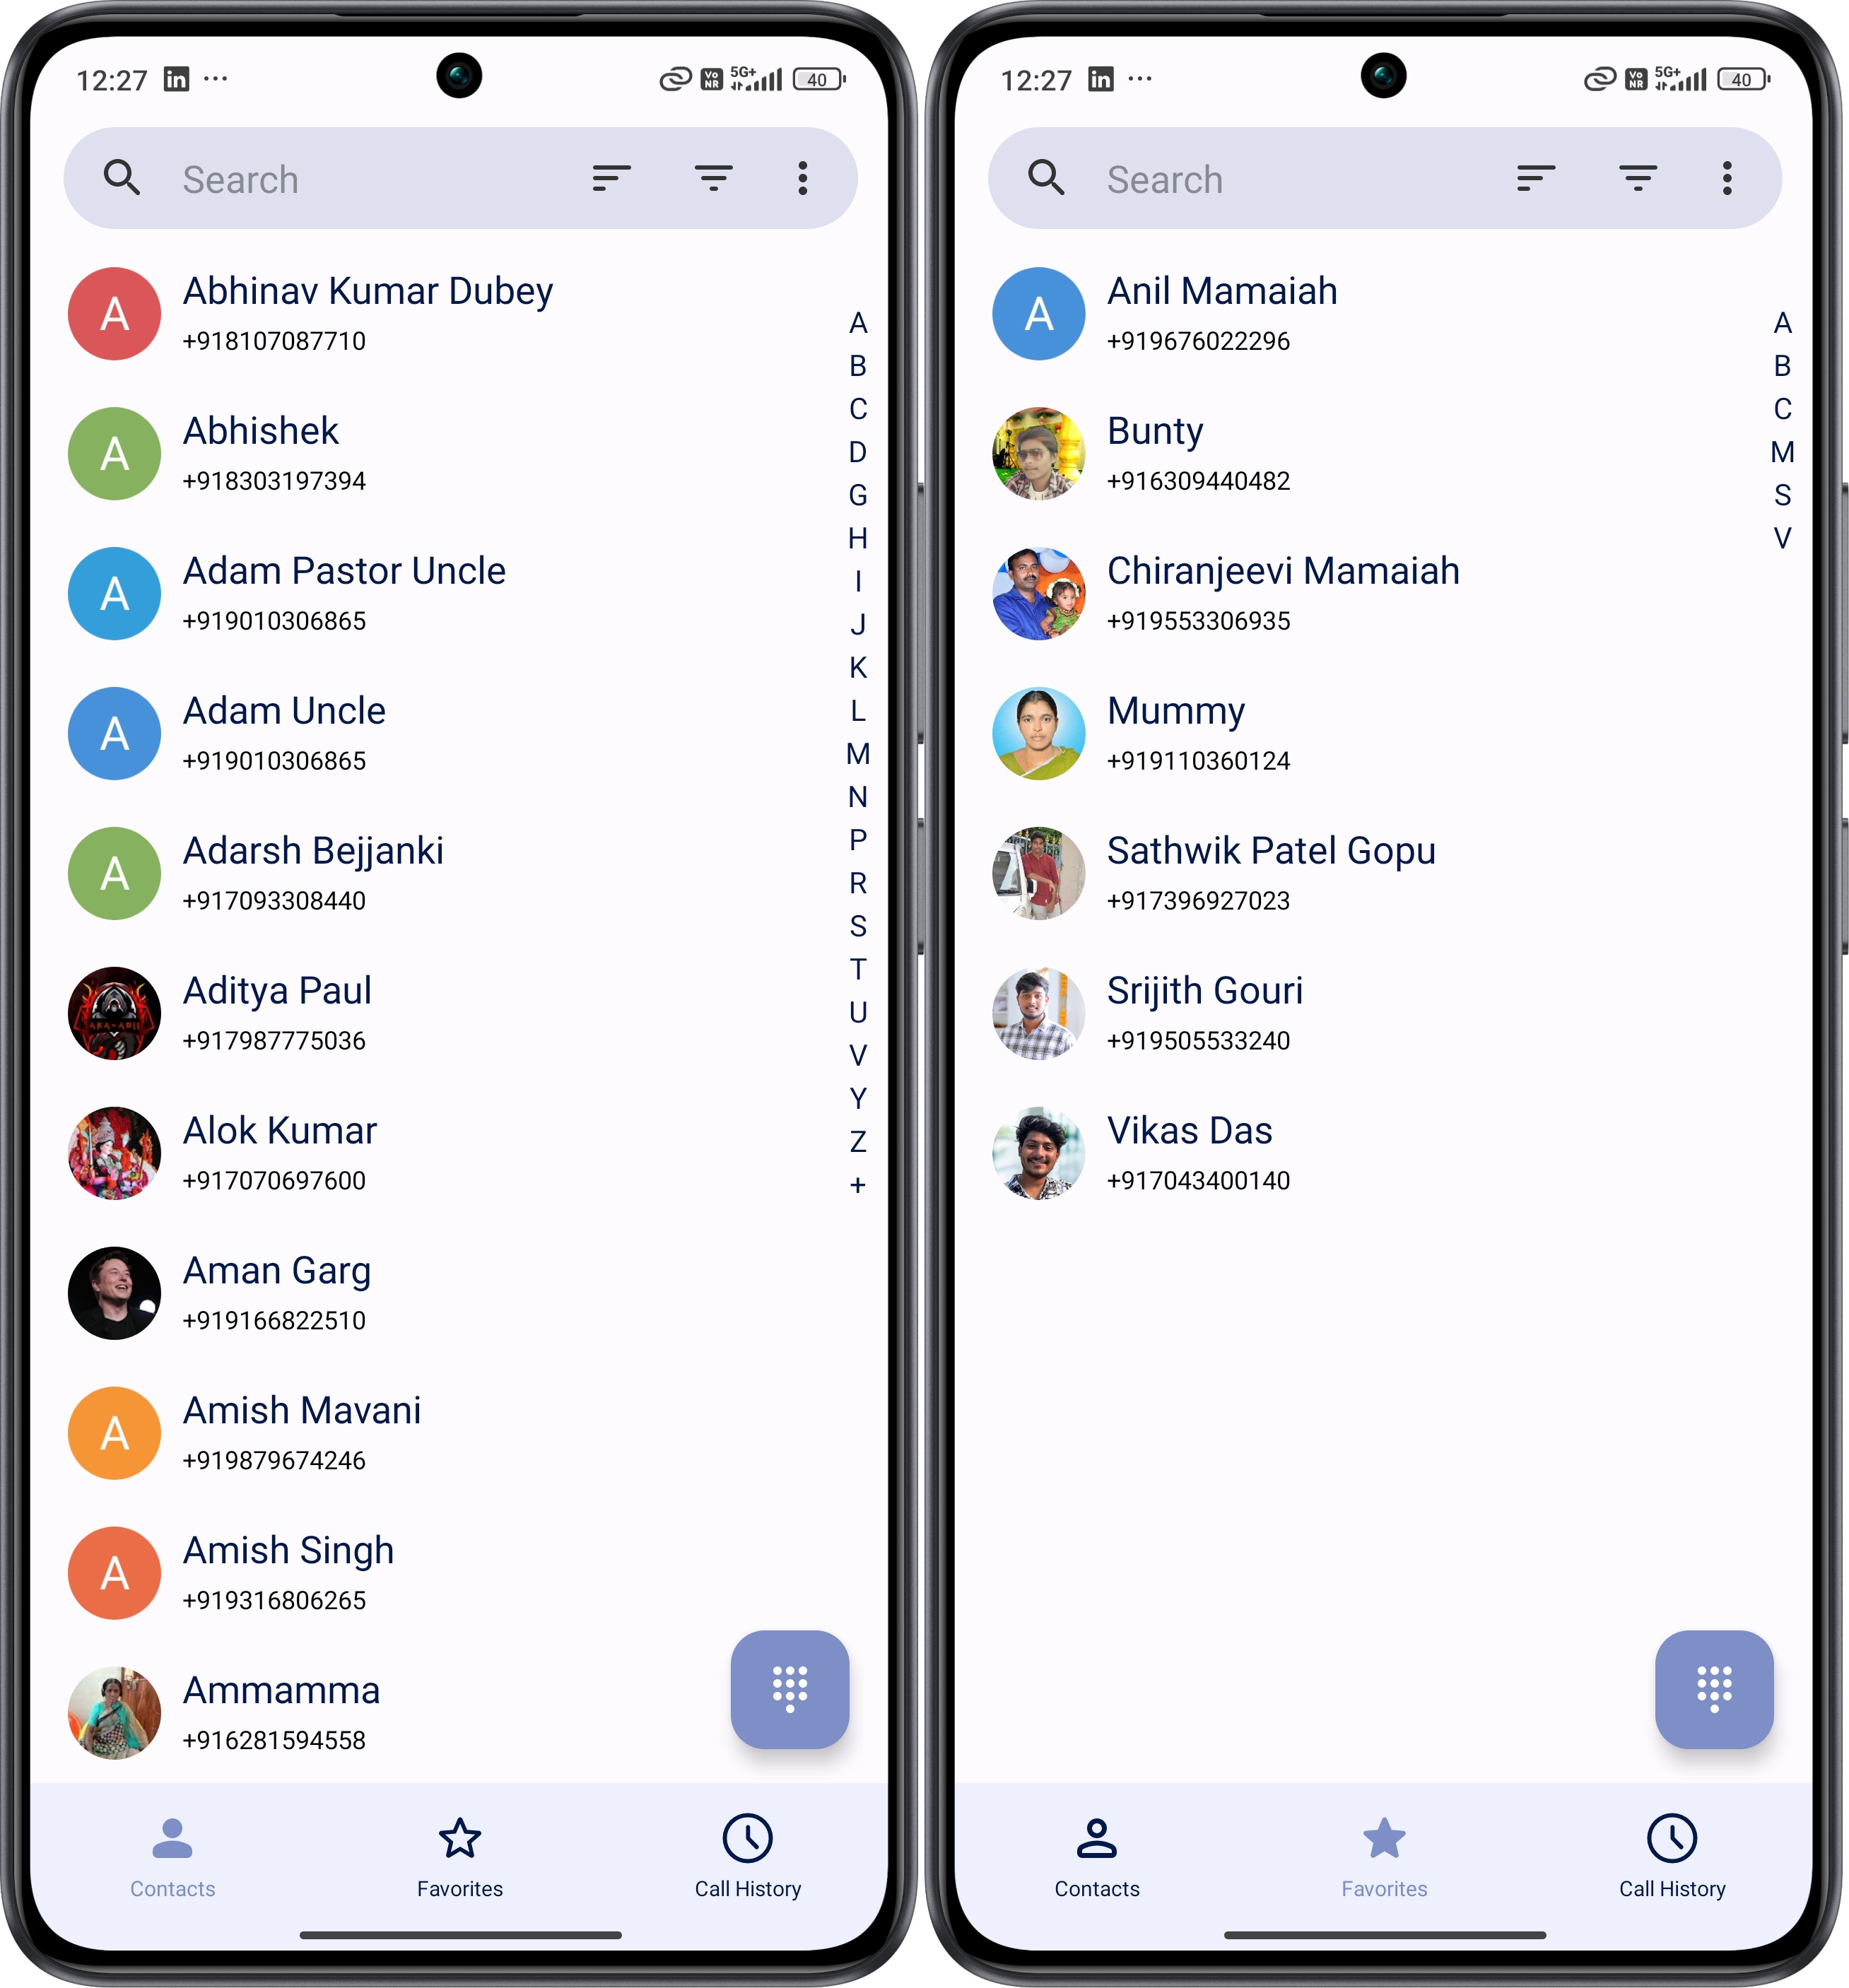
\includegraphics[width=1\linewidth]{Media//whatsapp/contactsand}
%    \caption{Contacts and Call logs Tabs}
%    \label{fig:Contacts and Call logs Tabs}
%\end{figure}
%
%\begin{figure}
%    \centering
%    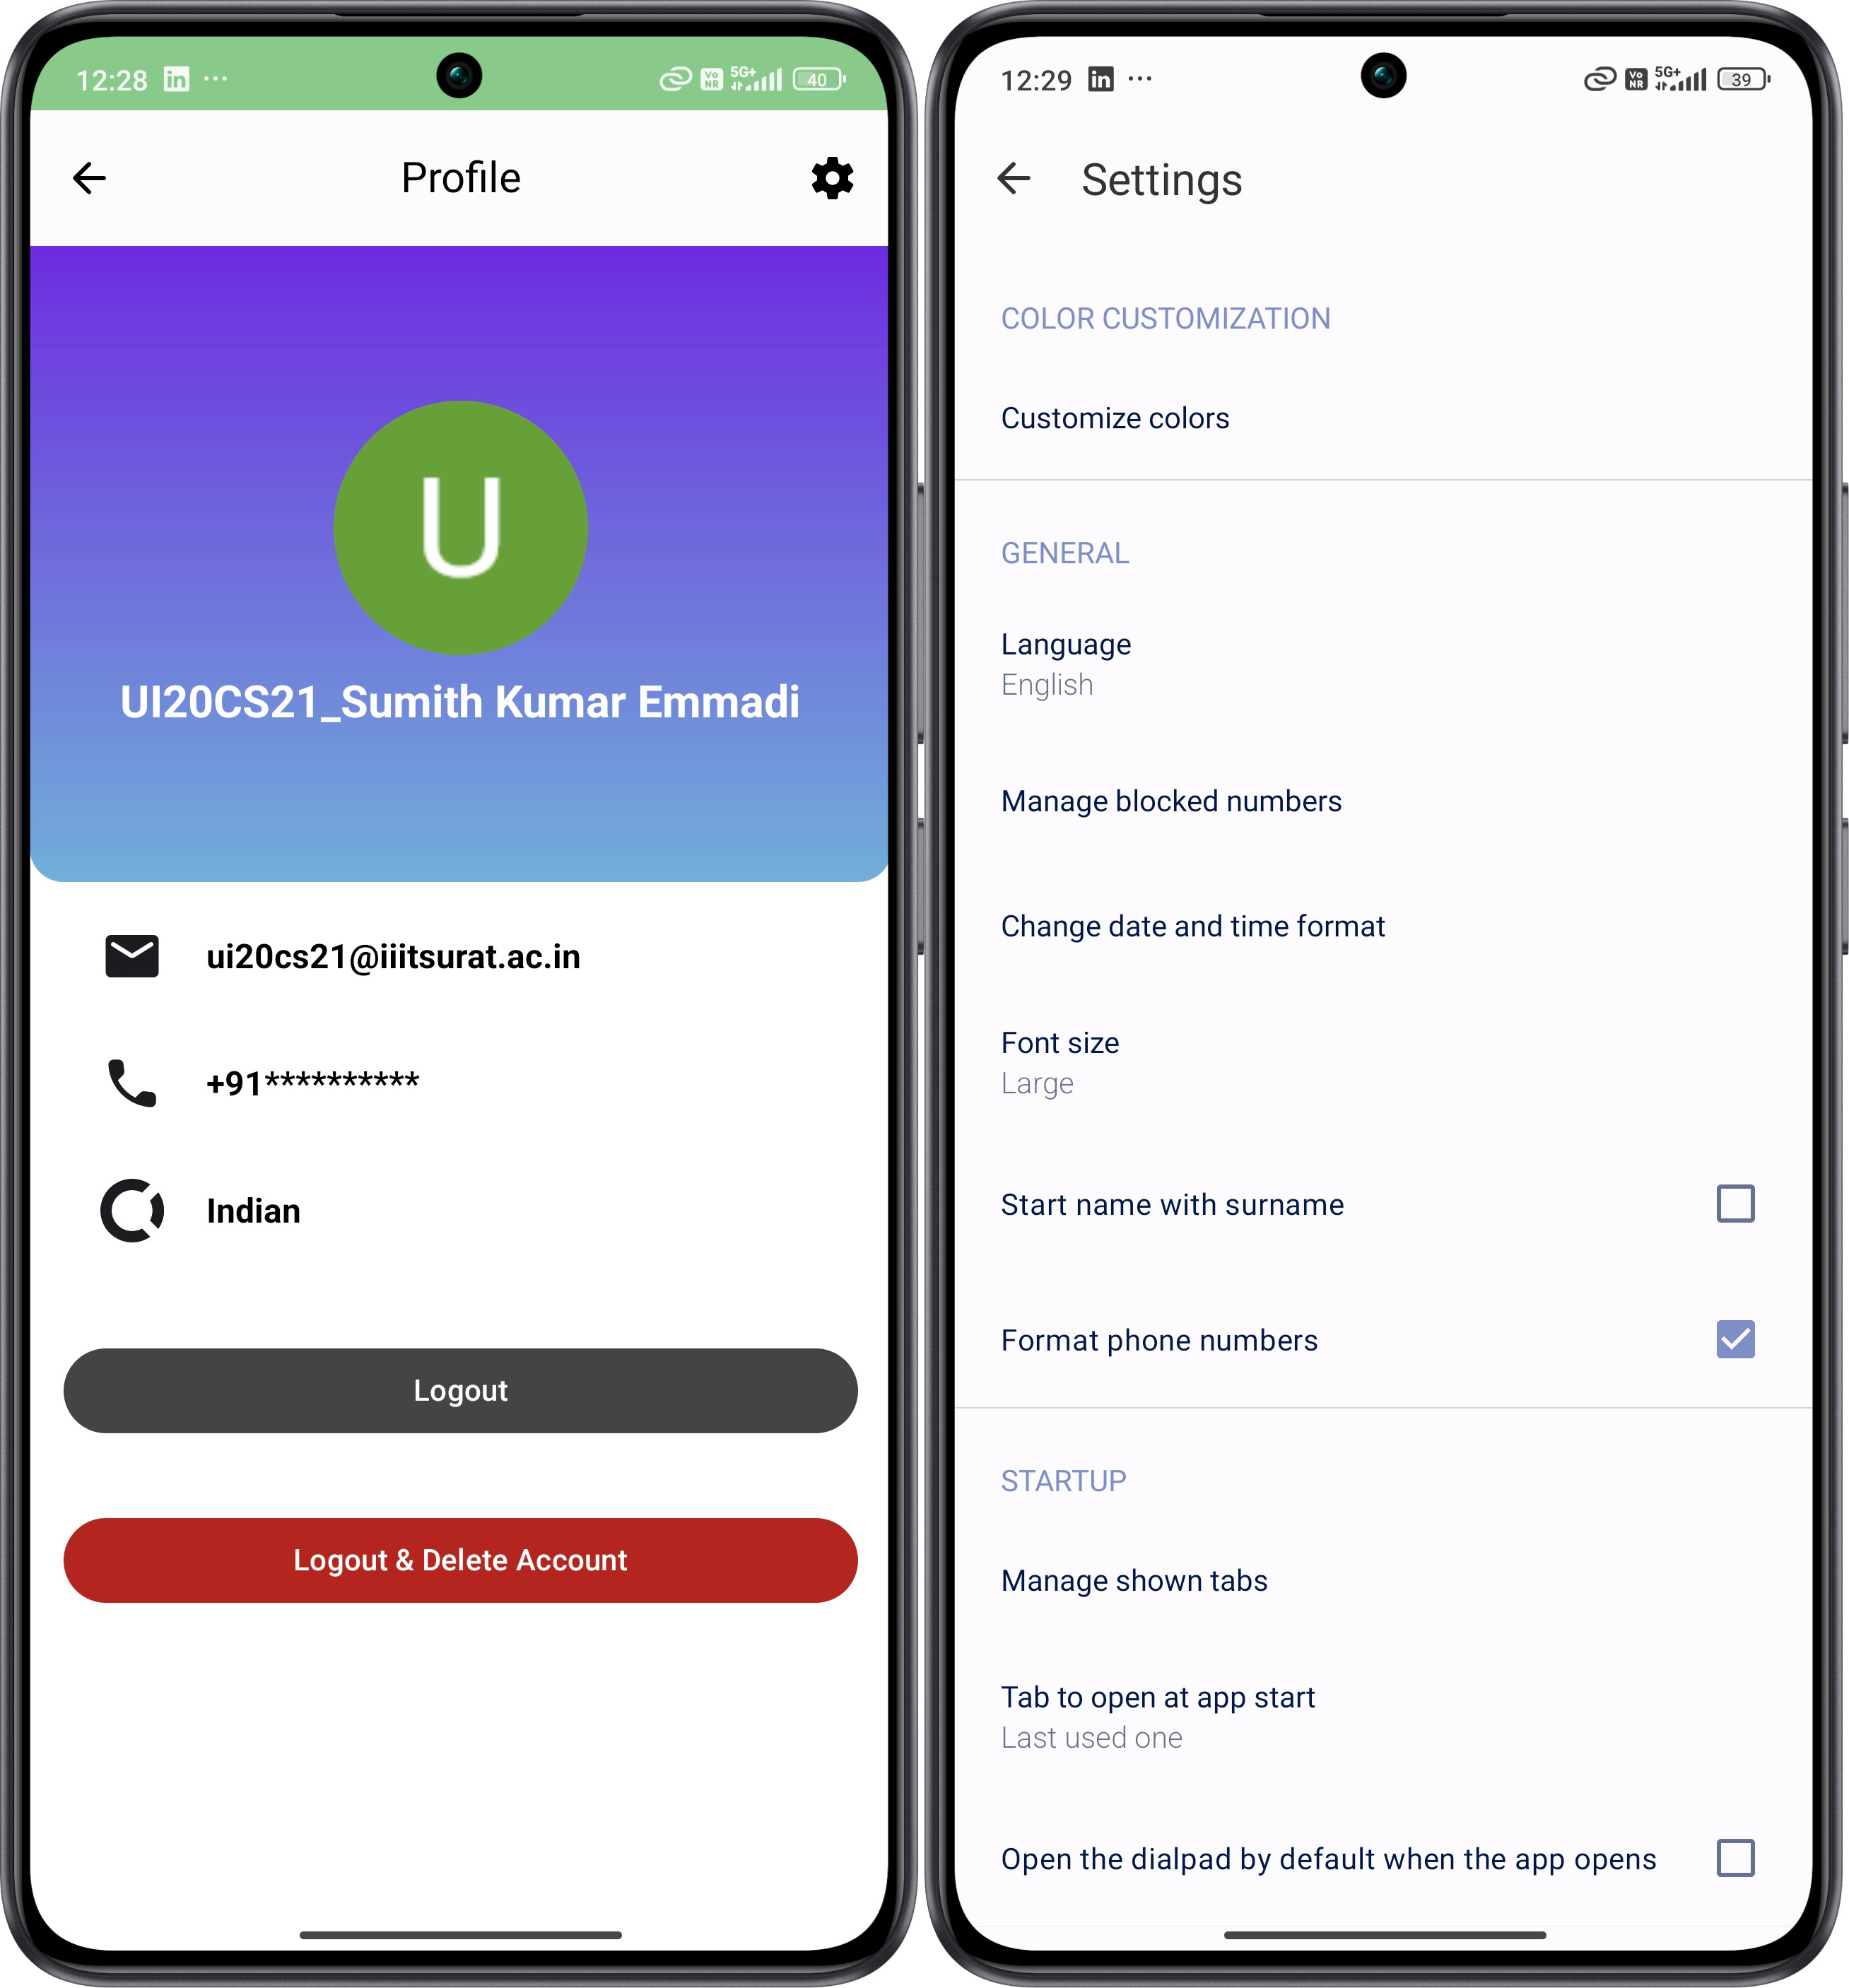
\includegraphics[width=1\linewidth]{Media//whatsapp/profile}
%    \caption{Profile and Settings}
%    \label{fig:Profile and Settings}
%\end{figure}
%
